\begin{marginfigure}
  \centering
  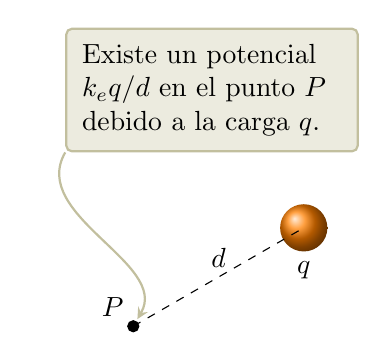
\begin{tikzpicture}[>=stealth]
    \coordinate (P) at (0,0);
    \shade[ball color=orange] (30:2.5) circle (.3) node[below=3mm] {$q$};
    \draw[dashed] (P) -- node[above] {$d$} (30:2.5);
    \filldraw (P) circle (2pt) node[above left] {$P$};
    \node (cartel) [
      text width=3.3cm,
      align=left,
      fill=yellow!40!black!14,
      draw=yellow!40!black!46,
      thick,
      rounded corners=2pt,
      inner sep=2mm
      ]
      at (1,3) {Existe un potencial $k_e q/d$ en el punto $P$ debido a la carga $q$.};
    \draw[->, thick, color=yellow!40!black!46, shorten >=3pt] 
             (cartel.south west) to[out=240, in=60] (P);
  \end{tikzpicture}
  \caption{Potencial en el punto \(P\) debido a \(q\).}
  \label{fig_potencial_en_un_punto}
\end{marginfigure}
